\section{Friday}\index{week3_Friday_lecture}

\newcommand{\HRule}{\rule{\linewidth}{0.5mm}}
\HRule \\[0.5cm]
{
\begin{center}
 \centering
\includegraphics[width=0.4\textwidth]{./logo}~\ 
 
\includegraphics[width=0.4\textwidth]{./logo_1}~\
 \end{center}
  \say{\textit{Our first quiz is at 1:30-2:20pm on September 30th. That is next Sunday. There will be around $5$ questions.}} \textit{the Grandpa said breezily,}
}

\HRule \\[0.5cm]
\subsection{Review}
This lecture will review the continuty of function. Let's start with some easy examples:
\[
f(x)=\left\{
\begin{aligned}
x,&\quad x\in\mathbb{Q}\\
-x,&\quad x\notin\mathbb{Q}
\end{aligned}
\right.
\]
This function is continuous nowhere expect for $x=0$.

\begin{definition}[Continuous]
Given a function $f:D\mapsto\mathbb{R}$
, 
\begin{itemize}
\item
we say $f$ is \emph{continuous} at $x_0\in D$ if for $\forall\varepsilon>0$, $\exists \delta:=\delta(\varepsilon,x_0) >0$ s.t. $|f(y) - f(x_0)|<\varepsilon$ for $\forall |y-x_0|<\delta$
\item
$f$ is continuous on $D$ if it is continuous at every point in $D$.
\item
If $\delta:=\delta(\varepsilon)$, i.e., $\delta$
 is independent of $x_0\in D$, then $f$ is said to be \emph{uniformly continuous} on $D$.
\end{itemize}
\end{definition}
\begin{remark}
The following statements are equivalent, you should show by yourself.
\begin{enumerate}
\item
$f$ is continuous
\item
If $\{x_n\}\to x_0$ as $n\to\infty$, then $\{f(x_n)\}\to f(x_0)$ as $n\to\infty$.
\item
$f^{-1}(\bm A)$ is open/closed if the set $\bm A$ is open/closed.
\end{enumerate}
\end{remark}

\begin{definition}[Compact]
A set $K$ is \emph{compact} (cpt) if for evey open cover of $K$, there exists a \emph{finite} sub-cover.
\end{definition}
\begin{remark}
The compactness has an important connection with continuity, e.g., the continuous function $f$ maps compact sets to compact sets.
\end{remark}
There is a useful way to determine whether a point is continuous at $f$, which will be discussed in this lecture.
\subsection{Continuity Analysis}
Let's raise some examples first. From these examples we can see that the proof of continuousness is non-trival.
\begin{example}
\begin{enumerate}
\item
Given a funciton
\[
f(x) = \left\{
\begin{aligned}
\sin\frac{1}{x},&\quad x\ne0\\
0,&\quad x=0
\end{aligned}
\right.
\]
From the graph we can see that $f$ oscillates heavily near zero point.
\begin{figure}[H]
\centering
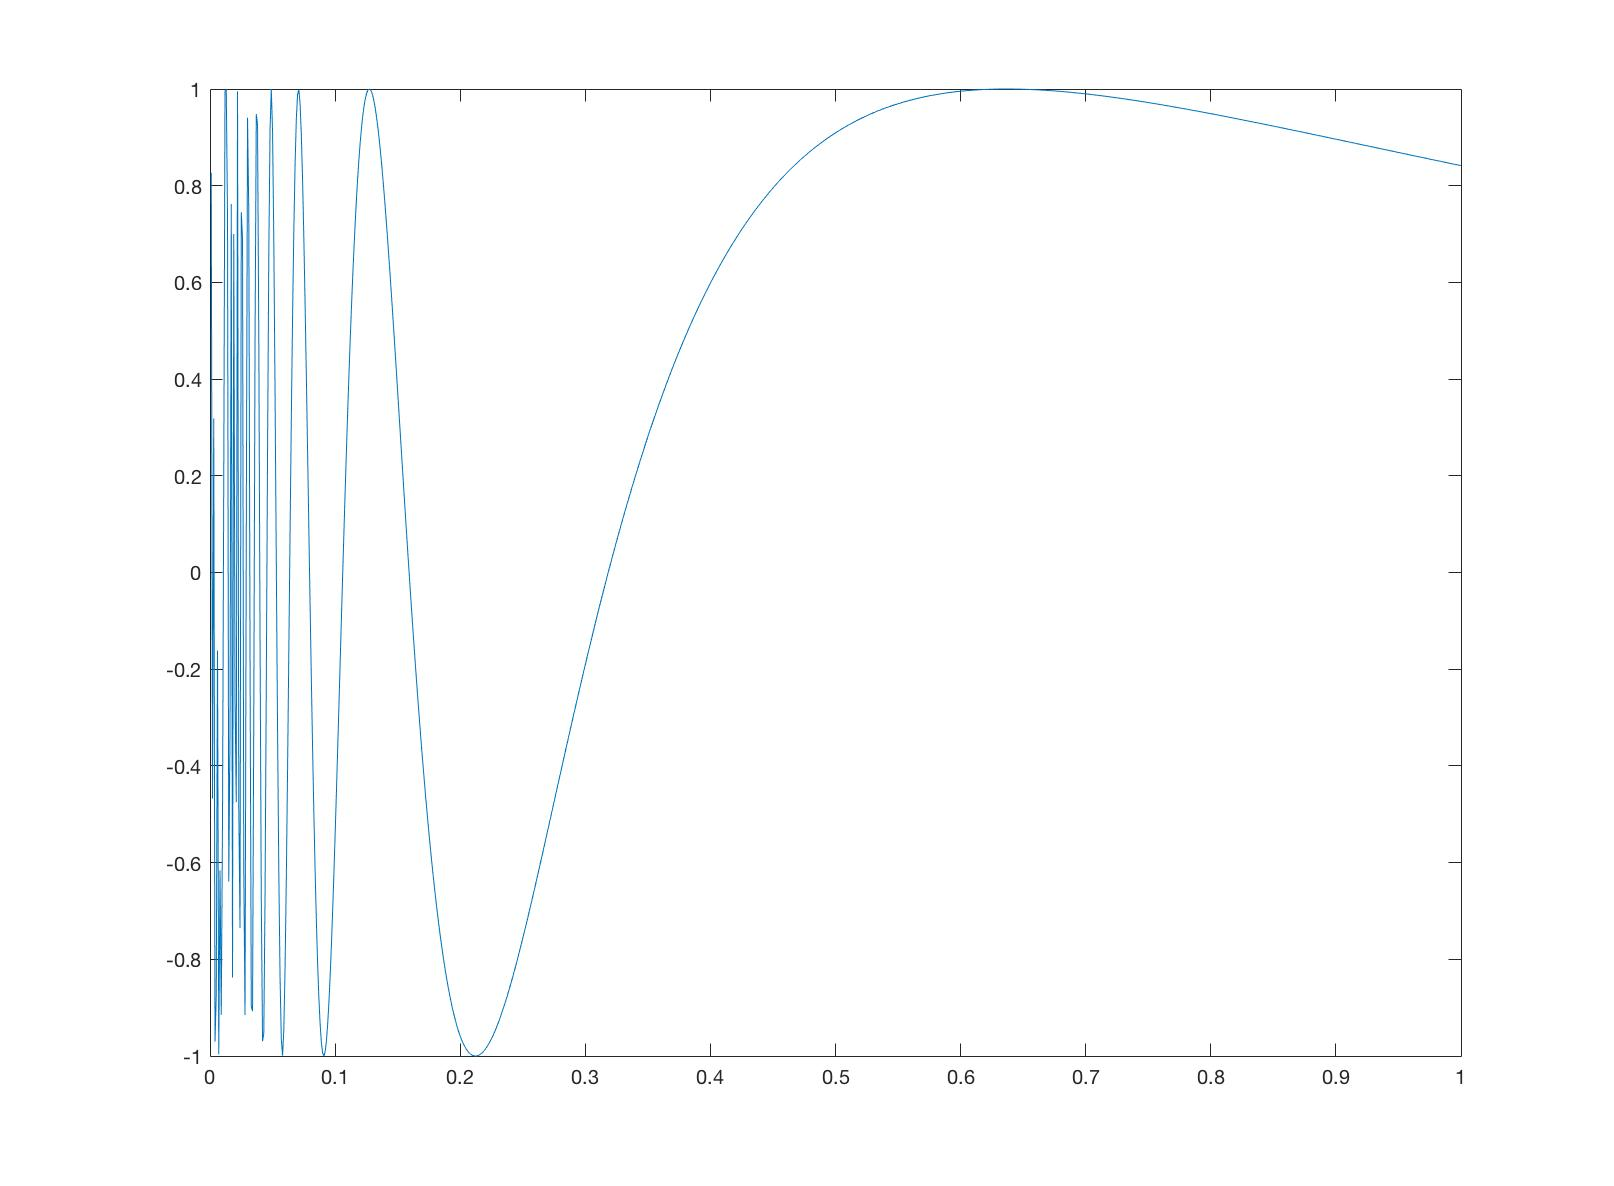
\includegraphics[width = 10cm]{3_F}
\caption{Graph for $f$}
\end{figure}

It is easy to show that $\sup_{x,y\in N_{\delta}(0)}|f(x) - f(y)|=2$ however small $\delta$ is.
\item
For another function
\[
g(x) = \left\{
\begin{aligned}
x\sin\frac{1}{x},&\quad x\ne0\\
0,&\quad x=0
\end{aligned}
\right.
\]
Conversely, it oscillates weakly near the zero point.
\begin{figure}[H]
\centering
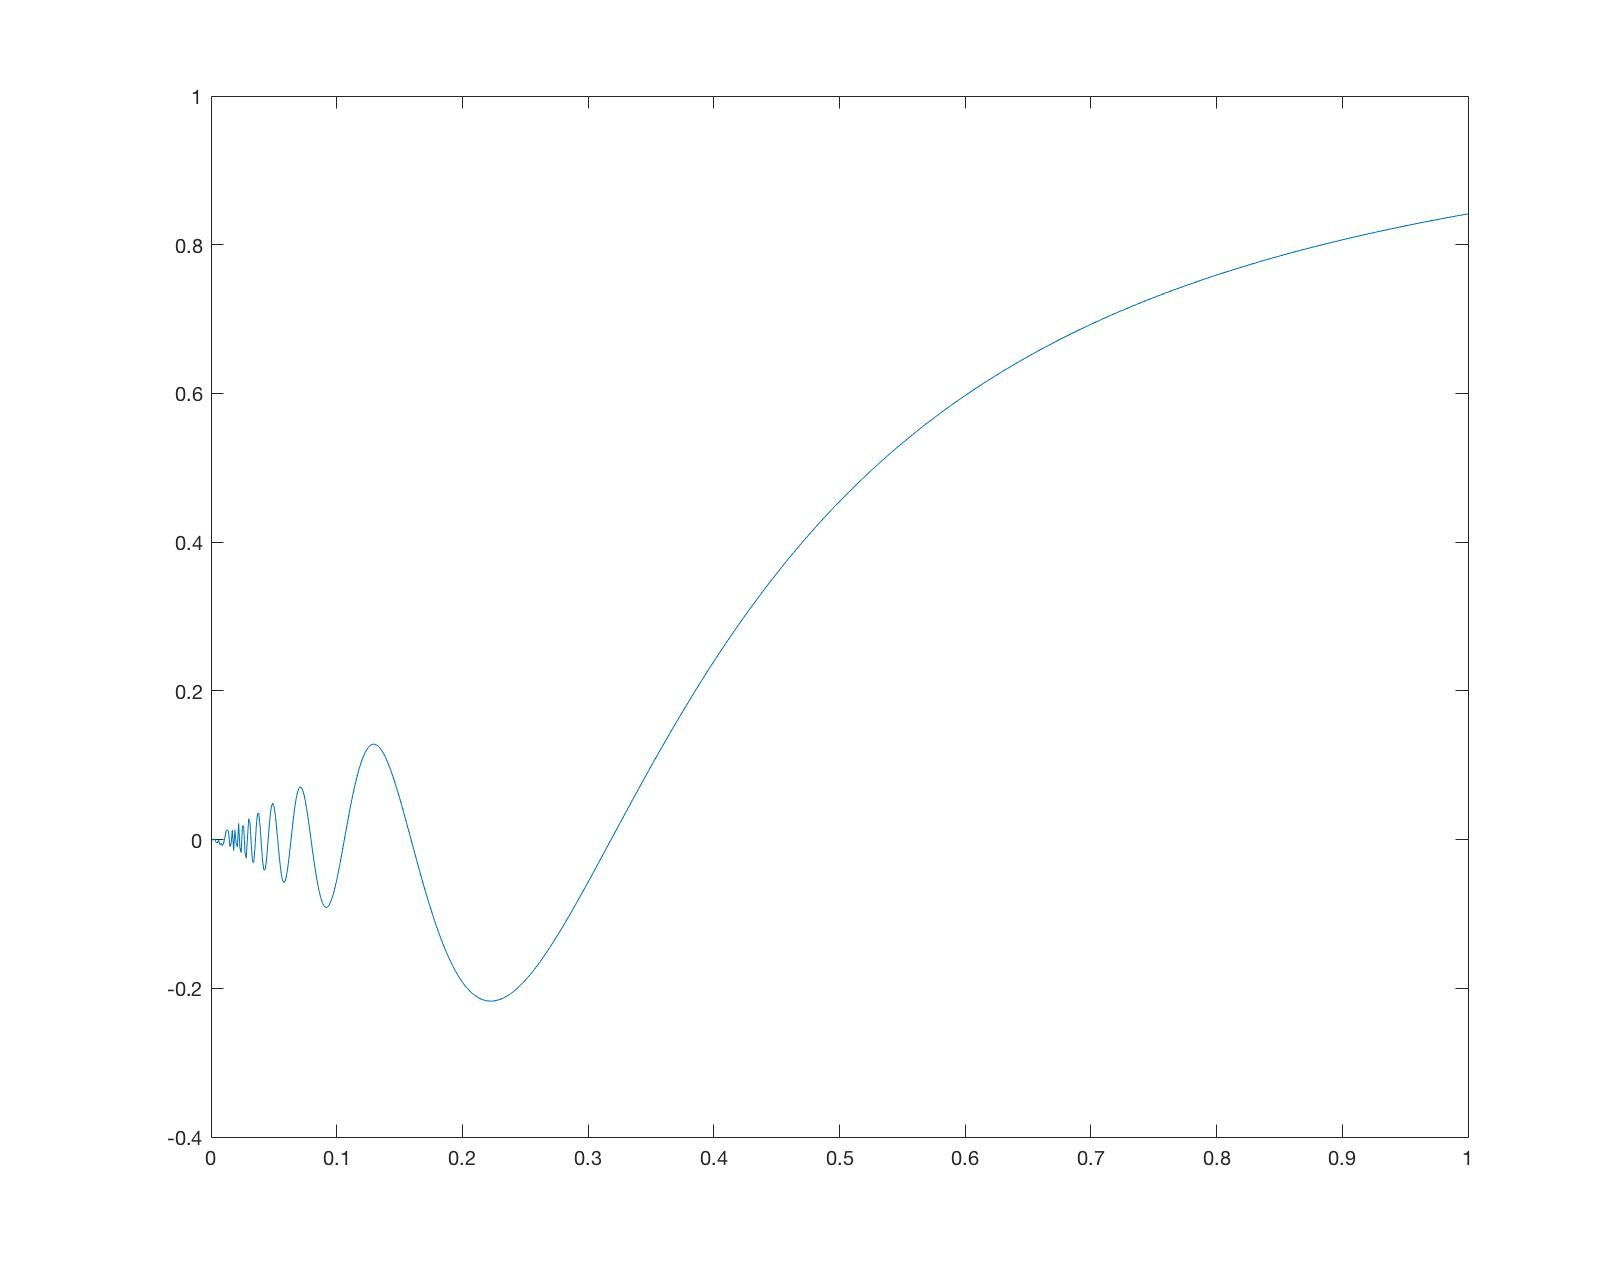
\includegraphics[width = 10cm]{3_G}
\caption{Graph for $g$}
\end{figure}
It is easy to show that $\sup_{x,y\in N_{\delta}(0)}|g(x) - g(y)|=0$ as $\delta\to0$.
\end{enumerate}
\end{example}
\begin{definition}[oscillation]
\begin{itemize}
\item
The oscillation of a function $f$ on $E$ is defined as
\[
\omega(f;E) := \sup_{x,y\in E}|f(x) - f(y)|
\]
\item
The oscillation of $f$ at a single point $x_0$ is defined as
\[
\lim_{\delta\to0}\omega(f,N_\delta(x_0)) := w(f;x_0)
\]
\end{itemize}
\end{definition}
\begin{remark}
\begin{itemize}
\item
Here we abuse the notation to denote the oscillation at $x_0$ with $\omega(f;x_0)$, but note that $\omega(f;x_0)\ne \omega(f;\{x_0\})$.
\item
The well-definedness of $w(f;x_0)$ is because $\omega(f,N_\delta(x_0))$ is non-incresing as $\delta$ decreases and has a lower bound $0$.
\item
A function $f$ is continuous at $x_0$ iff $w(f,x_0) = 0$. (verify by yourself)
\end{itemize}
\end{remark}
An classical example that illustrates a function can have continuous points in $\mathbb{R}\setminus\mathbb{Q}$ is shown below. We have faced this example in the diagnostic quiz:
\begin{example}
The Dirichlet function is defined for $\mathbb{R}\setminus\{0\}$:
\[
f(x) = \left\{
\begin{aligned}
0,&\quad x\notin\mathbb{Q}\\
\frac{1}{q},&\quad x=\frac{p}{q},q>0,(p,q)=1
\end{aligned}
\right.
\]
The function $f$ is continuous at $x$ iff $x\notin\mathbb{Q}$. 
The set of all discontinuous points of $f$ is $\mathbb{Q}$. 
\end{example}
Now the question turns out:
\begin{quotation}
\textit{
Does there exists a function $g$ of which the set of all discontinuous points of $g$ is $\mathbb{R}\setminus\mathbb{Q}$?
}
\end{quotation}

Applying Baire-Category Theorem, we will show the answer to this question is no.

\begin{proposition}\label{pro:3:2}
Suppose $f$ is continuous on a dense set in $\mathbb{R}$. Then the set of all discontinous points of $f$, denoted as $T$, must form a set of first category, i.e., (a countably union of nowhere dense sets)
\end{proposition}
\begin{remark}
$\mathbb{R}\setminus\mathbb{Q}$ is of second category, otherwise assume
\[
\mathbb{R}\setminus\mathbb{Q}=\bigcup_{i=1}^\infty I_i
\]
for nowhere dense sets $I_i$, which implies $\mathbb{R}=[\cup_{i=1}^\infty I_i]\bigcup[\cup_{q\in\mathbb{Q}}\{q\}]$ is a countably union of nowhere dense sets. Thus by applying proposition(\ref{pro:3:2}), the irrational number space cannot be the set of discontinuities.
\end{remark}

The idea of the proof is to express $T$ as countably union of sets, and argue that at least one of which must be nowhere dense.
\begin{proof}

We construct $D_n=\{x\in\mathbb{R}\mid w(f;x)\ge\frac{1}{n}\}$, which follows that
\[
T=\bigcup_{n=1}^\infty D_n.
\]
It suffices to show that $D_n$ is nowhere dense for every $n$ by contradiction.

Assume for some fixed $n$, $D_n$ is not nowhere dense, i.e., $\overline{D_n}$ contains an \emph{open} interval $\bm I$. Note that the set of continuous points is dense, we conclude that there exists a point $a$ inside the interval $\bm I$ such that $f$ is continuous at $a$. (why?) Also, there exists a sequence $\{b_k\}\subseteq D_n$ with limit $a$. (since you can verify $D_n$ is closed)

\begin{subequations}
Since $f$ is continuous at $a$, there exists $\delta>0$ such that 
\begin{equation}\label{Eq:3:3:a}
|f(x) - f(a)|<\frac{1}{4n} \mbox{for $|x-a|<\delta.$}
\end{equation}
At the same time $\{b_k\}\subseteq(a-\delta,a+\delta)$ for all large $k$, i.e., $\omega(f;b_k)\ge\frac{1}{n}$. Hence, there exists a sequence $\{c_{kl}\}$with limit $b_k$, such that the difference $|f(c_{kl}) - f(b_k)|$ is at least greater than $\frac{1}{2n}$ (why not $\frac{1}{n}$?), i.e., 
\begin{equation}\label{Eq:3:3:b}
|f(c_{kl} - f(b_k)|\ge\frac{1}{2n}
\end{equation}
Meanwhile, for large $l$, note that $c_{kl}$ is close to $a$, i.e., from (\ref{Eq:3:3:a}) we have
\begin{equation}\label{Eq:3:3:c}
|f(c_{kl}) - f(a)|<\frac{1}{4n}
\end{equation}
Also, note that $b_k$ is close to $a$ for large $k$, i.e.,from (\ref{Eq:3:3:a}) we have
\begin{equation}\label{Eq:3:3:d}
|f(b_k) - f(a)|<\frac{1}{4n}
\end{equation}
\end{subequations}
Three inequalities (\ref{Eq:3:3:b}) to (\ref{Eq:3:3:d}) show a contradiction: 
\[
|f(c_{kl}) - f(b_k)|\le |f(c_{kl}) - f(a)|+|f(b_k) - f(a)|<\frac{1	}{4n}+\frac{1}{4n}=\frac{1}{2n}
\]
\end{proof}

\begin{theorem}
Let $f$ be the \emph{pointwise} limit of a sequence of continuous functions $\{f_n\}$, i.e., $f(x) = \lim_{n\to\infty}f_n(x)$. Then the set if all discontinuous points of $f$ must be a set of first category.\label{The:3:3}
\end{theorem}
\begin{remark}
Review the uniform limit version of this theorem; 
\end{remark}
\begin{proof}
We claim $D_{\varepsilon} = \{x\in\mathbb{R}\mid \omega(f,x)\ge\varepsilon\}$ is nowhere dense for any $\varepsilon>0$. (fixed $\varepsilon$).

Assume $\overline{D_{\varepsilon}}$ contains an open set, or equivalently, $D_{\varepsilon}$ contains an open set $\mathcal{U}$(since $D_{\varepsilon}$ is closed, i.e., $\overline{D_{\varepsilon}}=D_{\varepsilon}$). Define 
\[
A_{mn} = \left\{x\in U\mid |f_m(x) - f_n(x)|\le\frac{\varepsilon}{4}\right\}.
\]
\begin{proposition}
The set $A_{mn}$ is closed.
\end{proposition}
The proof of proposition is moved in the end.

Set $A_m = \bigcap_{n\ge m}A_{mn}$, which is also closed, and 
\[
A_m\subseteq\left\{x\in U\mid |f_m(x) - f(x)|\le\frac{\varepsilon}{4}\right\}
\]

For every $x\in U$, as $\lim_{n\to\infty}f_n(x)=f(x)$, we have $x\in\bigcup_{m=1}^\infty A_m$, which implies $U\subseteq \bigcup_{m=11}^\infty A_m$. Applying the Baire Category Theorem, there exists one $A_m$ containing an open set $W$.

\begin{subequations}
For $x_0\in W\subseteq\mathcal{U}\subseteq D_{\varepsilon}$, pick $\{x_n\}\subseteq W$ with limit $x_0$ such that 
\begin{equation}
|f(x_n) - f(x_0)|\ge\frac{3}{4}\varepsilon\label{Eq:3:4:a}
\end{equation}
At the same time, since $x_n,x_0\in W$, it follows that
\begin{align}
|f_m(x_n) - f(x_n)|\le\frac{\varepsilon}{4}\\
|f_m(x_0) - f(x_0)|\le\frac{\varepsilon}{4}\label{Eq:3:4:c}
\end{align}
From (\ref{Eq:3:4:a}) to (\ref{Eq:3:4:c}), we conclude that
\begin{align*}
\frac{3}{4}\varepsilon&\le
|f(x_n) - f(x_0)|\\&\le
|f_m(x_n) - f(x_n)|
+
|f_m(x_n) -f_m(x_0)|
+
|f_m(x_0) - f(x_0)|\\
&\le
\frac{1}{2}\varepsilon+|f_m(x_n) -f_m(x_0)|
\end{align*}
Or equivalently,
\begin{equation}
|f_m(x_n) -f_m(x_0)|\ge\frac{\varepsilon}{4},\forall n
\end{equation}
which implies $\omega(f_m;x_0)\ge\frac{\varepsilon}{4}$, which implies $f_m$ is discontinuous at $x_0$, which is a contradiction.
\end{subequations} 
\end{proof}
\begin{remark}
\begin{itemize}
\item
The proof for $A_{mn}$ is closed is easy: pick any sequence $\{x_k\}\subseteq A_{mn}$ with limit $x$, it suffices to show $x\in A_{mn}$, i.e., 
\[
\lim_{k\to\infty}|f_m(x_k) - f_m(x_k)|\le\frac{\varepsilon}{4}
\]
\item
The applications of Baire Category Theorem give us an estimation of how large and how small a set is. In next lecture we will see how large is the set of continuous but nowhere differential functions.
\end{itemize}
\end{remark}














